\providecommand{\todo}[1]{\textbf{[TODO: #1]}}

\section{Method}
\label{sec-method}

\begin{figure}[t]
\centering
\begin{minipage}[c]{0.57\linewidth}\centering
\textbf{A}\\[2pt]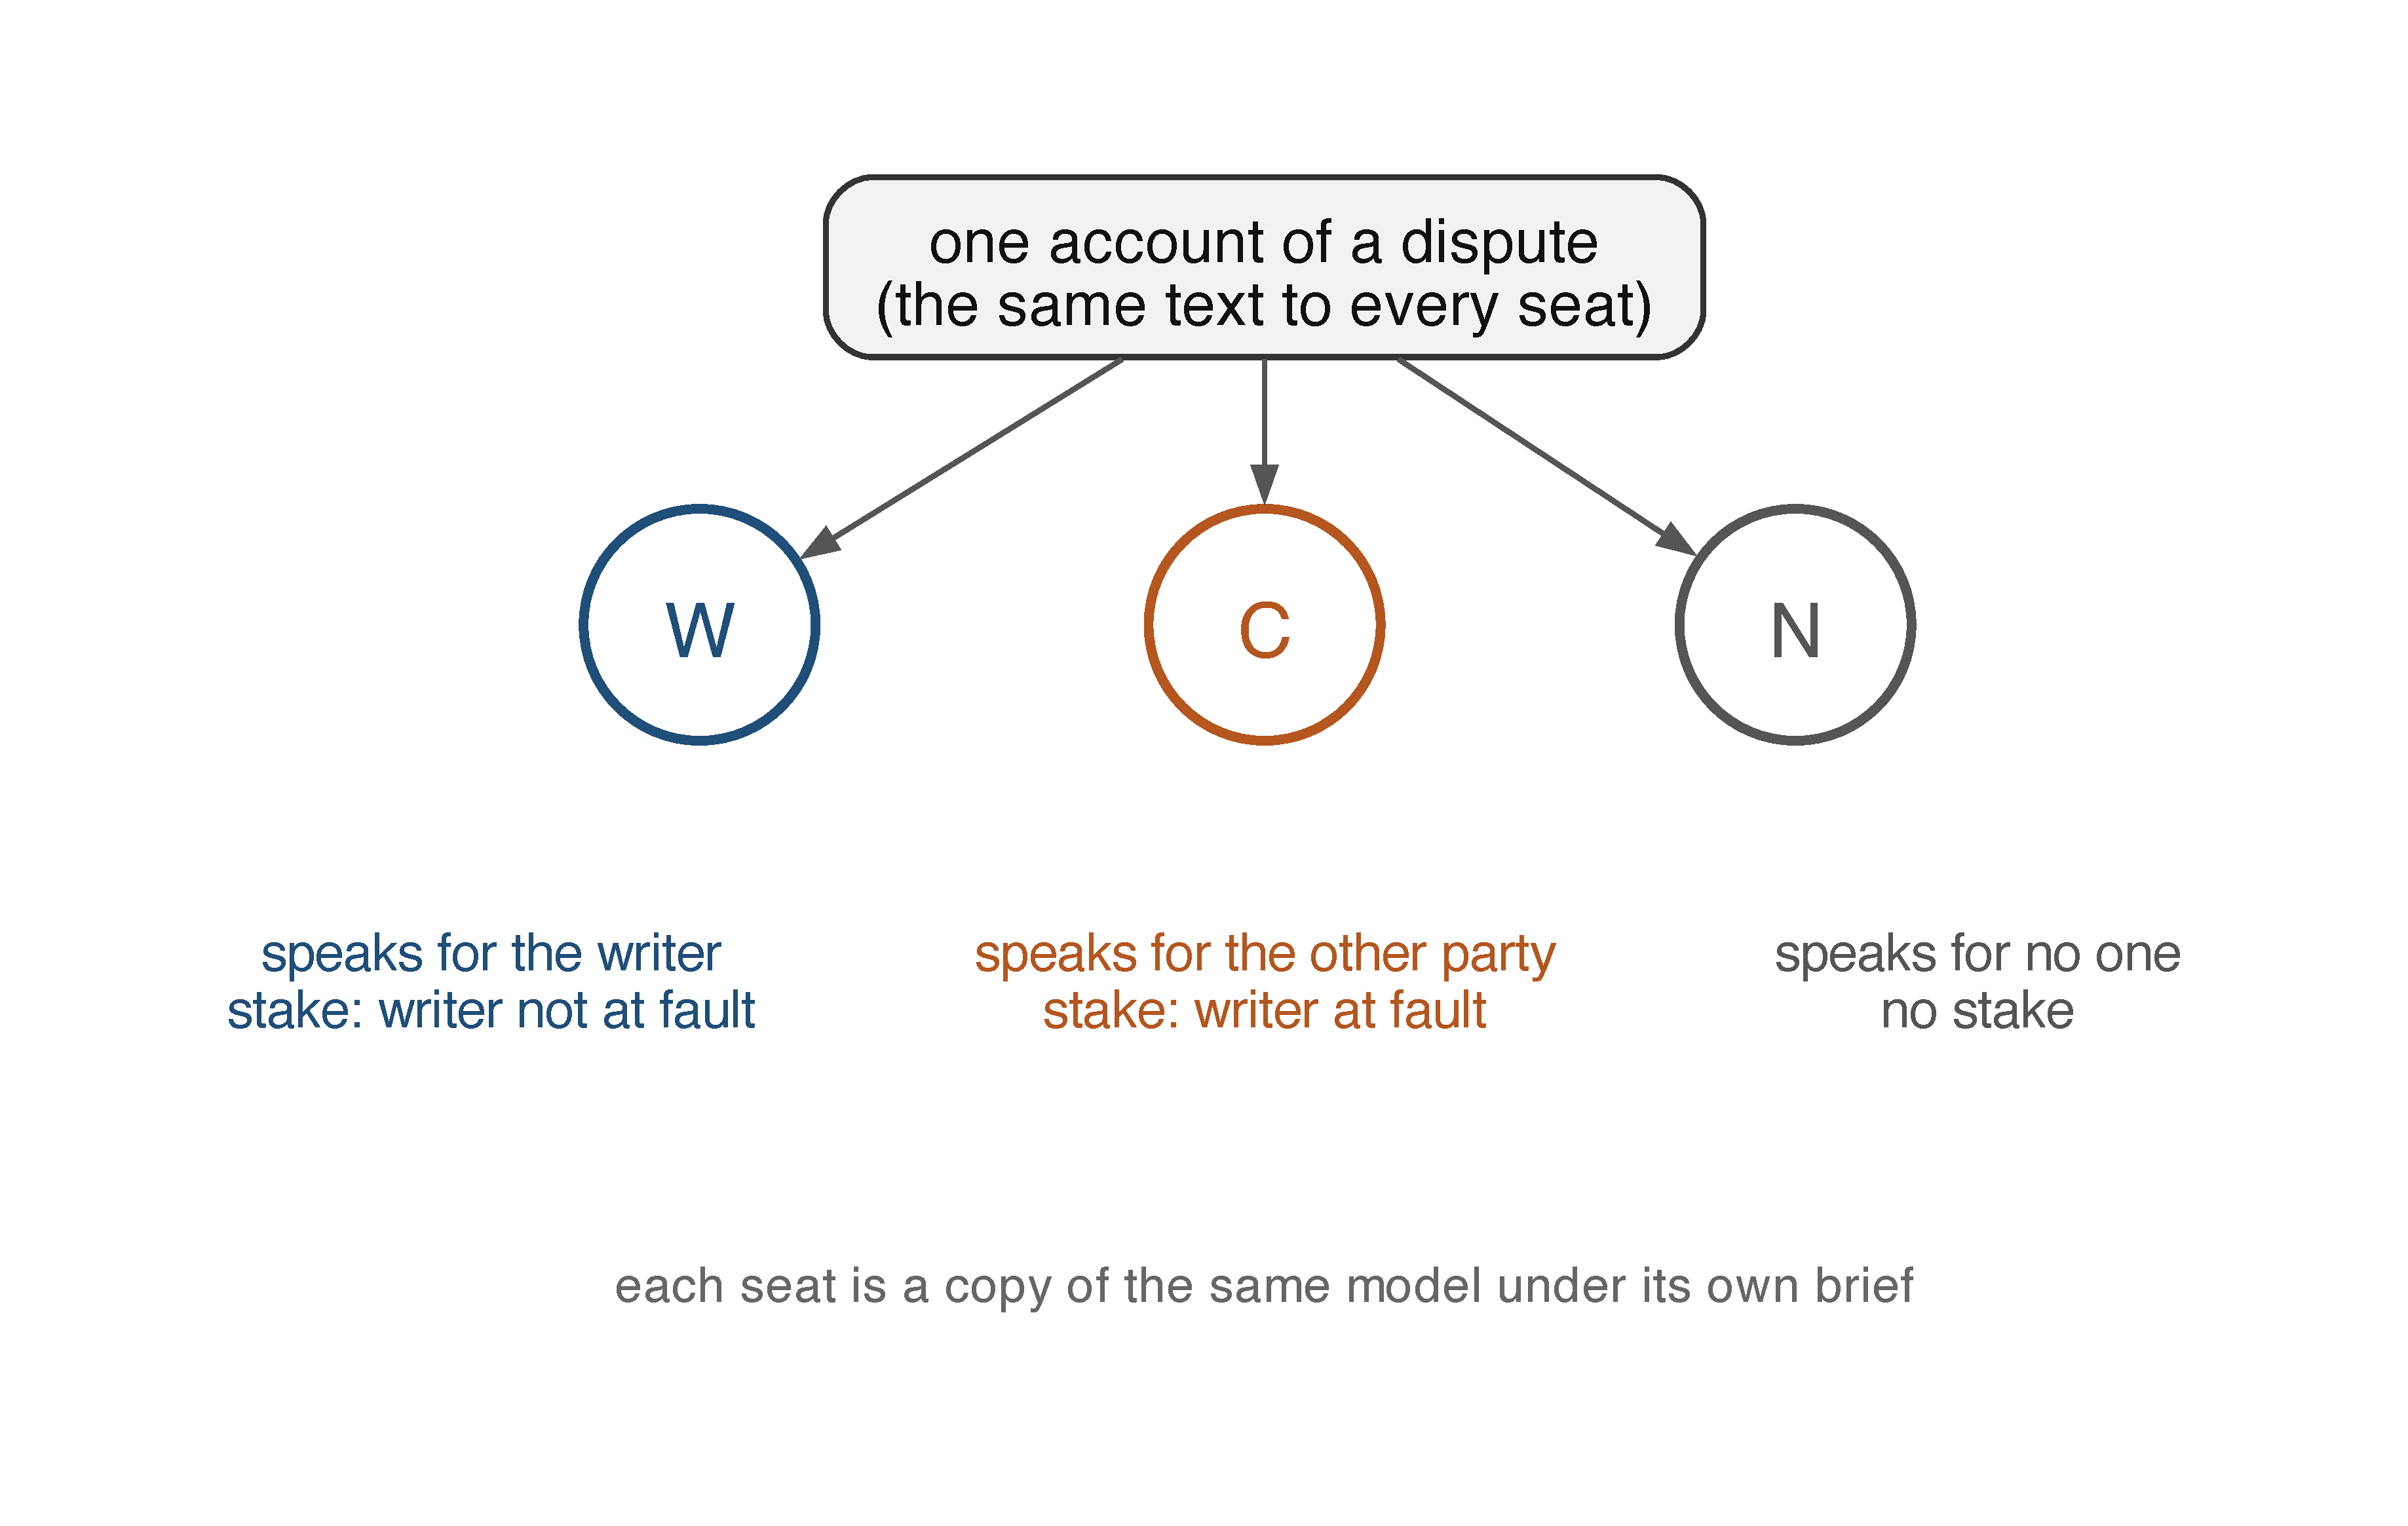
\includegraphics[width=\linewidth]{figures/fig_mechanism_a.pdf}\\[10pt]
\textbf{C}\\[2pt]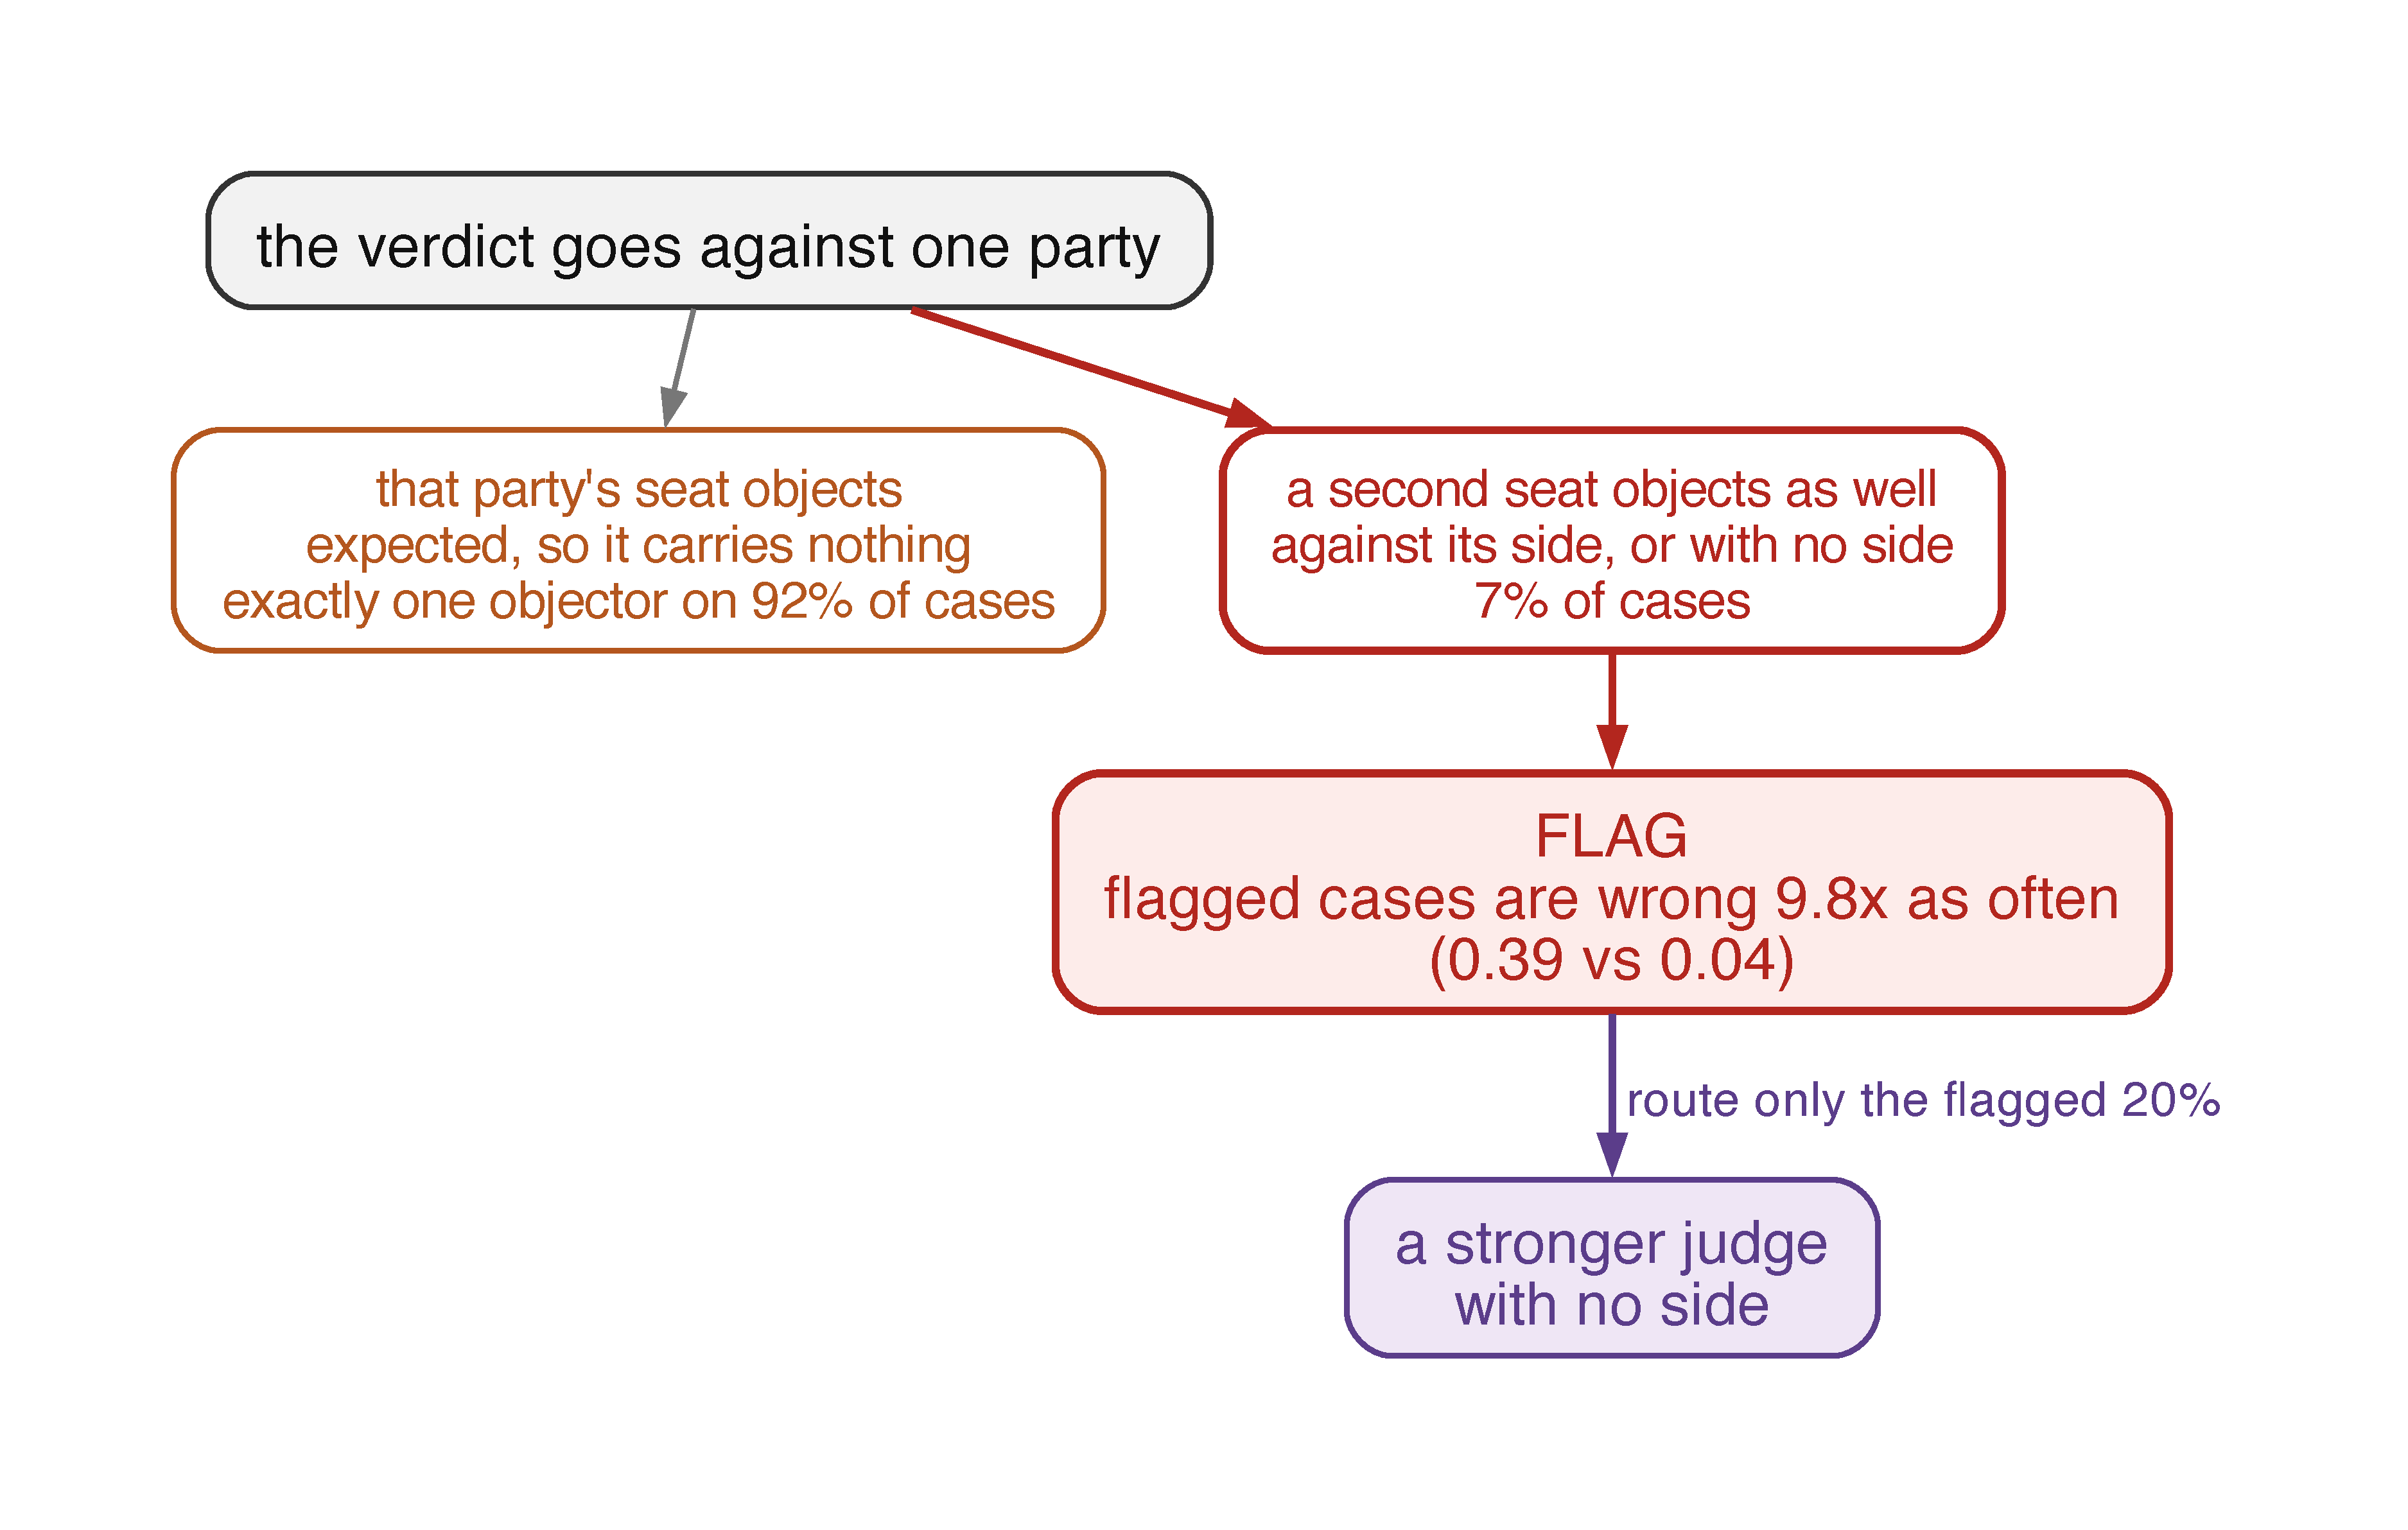
\includegraphics[width=\linewidth]{figures/fig_mechanism_c.pdf}
\end{minipage}\hfill
\begin{minipage}[c]{0.39\linewidth}\centering
\textbf{B}\\[2pt]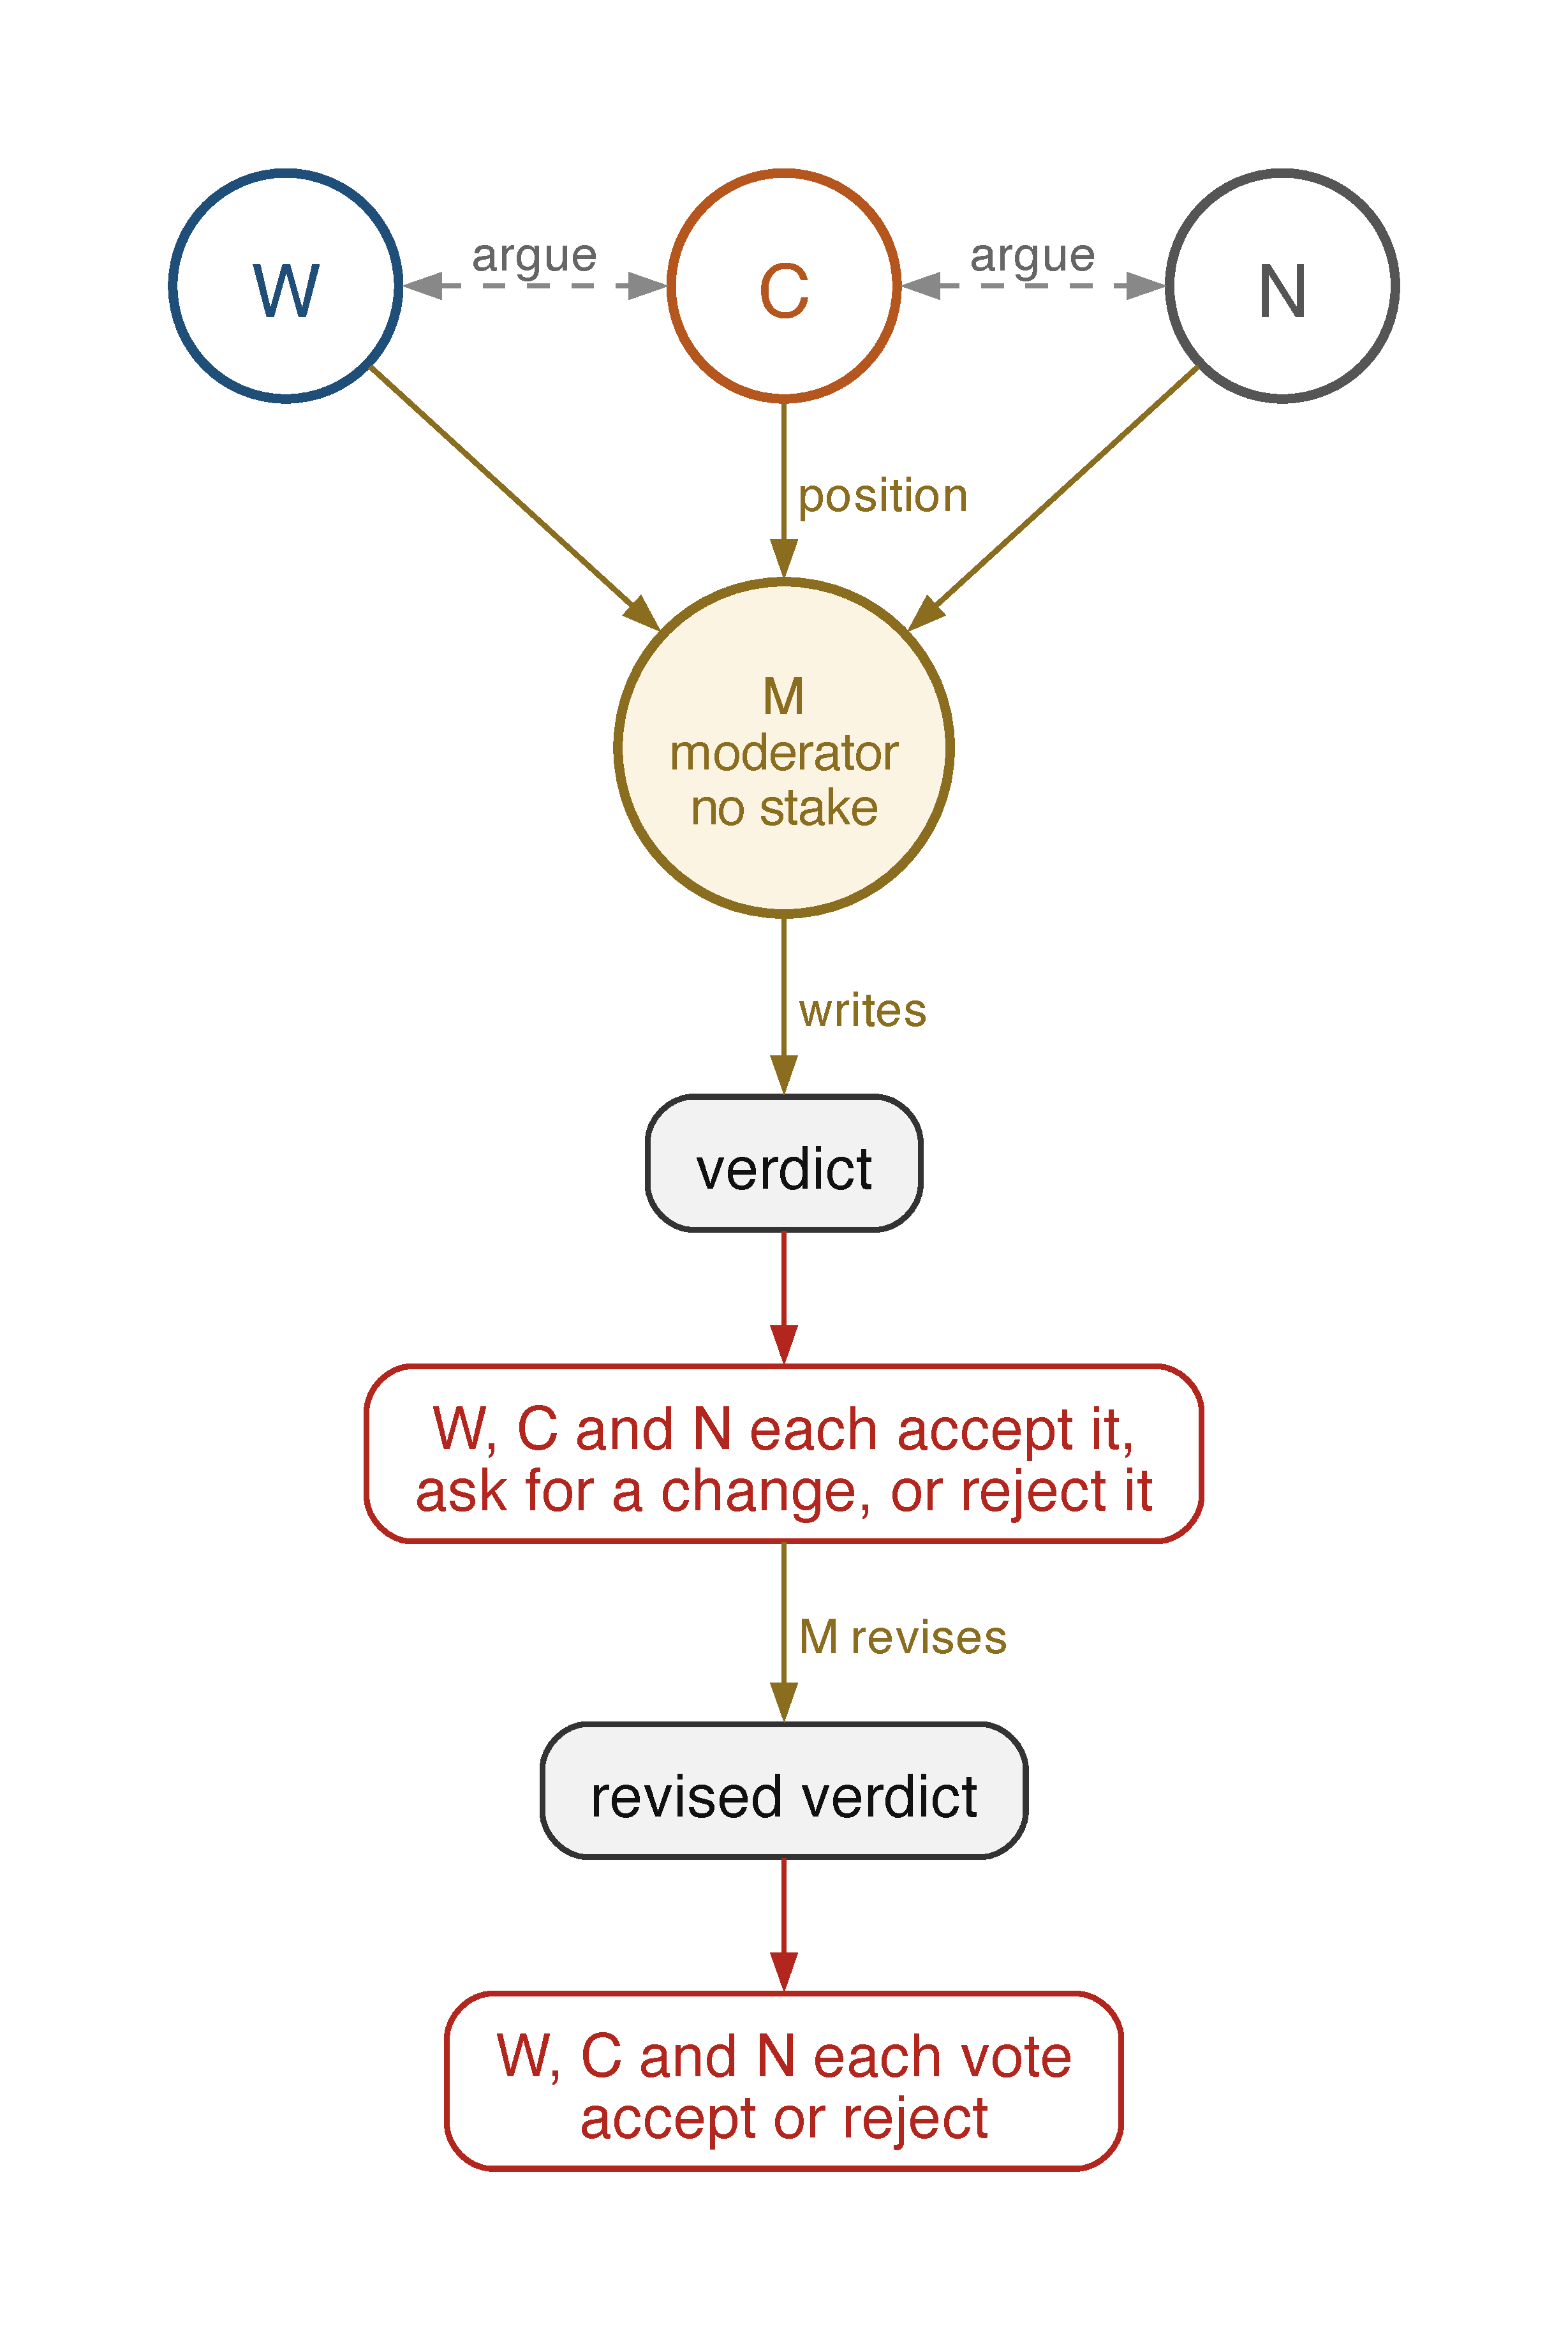
\includegraphics[width=\linewidth]{figures/fig_mechanism_b.pdf}
\end{minipage}
\caption{(A) Three copies of one model read one account, briefed for the
writer, the other party or no one. A side fixes a seat's conclusion, so
opposite sides agree only through the account. (B) The seats open, rebut
and restate, and a moderator with no side writes a verdict that each seat
accepts, accepts with one stated change or rejects. (C) The losing party's
seat is expected to object. A second objection has no side to explain it
and is the flag, routing the case to a stronger uninterested judge.}
\label{fig-mechanism}
\end{figure}

\subsection{Embodiment as a control}
\label{sec-method-embodiment}
\label{sec-method-interventions}

A seat is a copy of one model reading the account under a brief that
names whom it speaks for and what it wants
(Figure~\ref{fig-mechanism}A).
We chose a side over a persona because a persona changes how a copy
speaks and a side fixes what it concludes, which makes it a control.
Told it speaks for the writer, a copy finds the writer not at fault on
99.7 percent of opening statements, and for the other party, at fault on
97.4
percent.
Two seats hold opposite sides because what two locked seats agree on
came from neither brief and must come from the account
\citep{milgrom1986relying,dewatripont1999advocates}.
A third seat has no side because the verdict layer needs one uninterested
reader, and where the sides lock it is the seat any vote returns and the
best seat (Section~\ref{sec-results}).
Neither advocate may invent facts, and the writer's seat may not assert
that the writer is not in the wrong where the account does not support
it, so no objection can rest on what the account lacks. Provability need
only be partial, since a decider who knows the speakers' interests
conflict can count on one to correct a mistaken inference
\citep{lipman1995robust}.
Every seat narrates before it commits, the light dose, under the model's
own scaffold so arrangement is the only
difference.
Removing it later showed it amplifies a second seat's objection without
creating the pattern.
The writer's brief treats a finding against the writer as a finding
against its party and puts the case as strongly as the account allows. The
other party's brief treats a finding for the writer as a finding against
its party, one that did not write the account and cannot add to it, and
puts that case as strongly as the writer's own account allows. The
neutral brief speaks for everyone who will read the verdict and wants only
the finding the account supports.

\subsection{The collective as a graph}
\label{sec-method-collective}

An arrangement of seats is a graph, its nodes the seats and a moderator,
its edges who reads whom (Figure~\ref{fig-mechanism}B), three copies of
one model running seven stages in seventeen
calls.
Each seat opens alone with a position and a verdict, so lock is measured
first.
Each then rebuts the other two and restates a final position, the only
stages where seats read one another, six edges the no-edge control
cuts.
A moderator, a separate node with no stake, reads the account and the
three final positions and writes one synthesis and verdict, separating
arguing from
deciding.
It is the seats' model by default, so the collective adds only an
arrangement, and was varied later because nothing in the design fixes who
decides.
At the objection round each seat accepts the synthesis, accepts it with
one stated modification, or rejects it naming the concern no integration
could
absorb.
A stated change is required because the synthesis is the first concrete
proposal there is to change, because integration must answer something,
and because a seat that accepts once its own change is addressed has
revised rather than opined. An objection without one is a counted
parse
failure.
The moderator then integrates, saying whose request each part answers,
and each seat votes accept or
reject.

A moderator decides rather than a vote because where the sides lock a
vote adds nothing. Two fixed opposite verdicts cancel, so the majority is
the neutral seat's verdict, any weighting
\citep{shapley1984optimizing} can only reweight two constants, and three
draws of one model lack the independent errors a jury theorem needs
\citep{ladha1992condorcet}.
The moderator is instead the node whose verdict the seats criticise
\citep{mercier2011argumentative,longino1990science}, sitting off the
argument because a network converges only when no node dominates it
\citep{golub2010naive}.
Across cells the item text, verdict instruction and briefs are
byte-identical except for what a control varies, so cells differ only in
arrangement.

\subsection{The flag}
\label{sec-method-flag}

Suppose the verdict goes against one party (Figure~\ref{fig-mechanism}C).
Only that party's seat has reason to object, and that expected objection
says nothing about whether the verdict is right. A second objection comes
from the seat whose side won or the seat with none. No brief put it there,
so it must come from the account, and an admission against interest is
what a listener who knows only the interests can trust
\citep{milgrom1986relying,lipman1995robust}.
On one-loser verdicts exactly one seat objects on 92 percent of debates,
two or more on 7
percent.
As implemented the flag is a stake-blind count, firing when at least two
of the three seats, the uninterested seat included, object at the
objection round.
An earlier stake-aware composite, firing on the neutral seat's objection
or an advocate's against interest, needs each seat's stake and the
verdict's direction, which the plain count matches without
either.
Because the flag marks debates most likely to be wrong, a stronger
uninterested judge is paid for only there, answering flagged cases cold
by majority of three samples, ties to the
collective.
The flag needs a verdict with one loser, a hypothesis about the verdict
rather than the model, and fails by design in three settings. A verdict
blaming both parties or neither gives both sides reason to object and it
floods. Seats that never leave their sides give no second objection and
it is silent. A plan every party gains from has no loser and nothing to
read.

\subsection{Controls that isolate each decision}
\label{sec-method-controls}
\label{sec-method-designs}

Each decision was tested by removing or varying it, everything else held
at the registered protocol, further departures disclosed in the record,
outcomes in
Section~\ref{sec-results}.
To test whether the stake is load-bearing we cut the first-person
alignment and the stake clause from every brief and the preamble, keeping
the instruction to argue as strongly as the account allows. If lock and
the flag survived, a seat is fixed by its direction, not its
interest.
To test whether opposed sides are load-bearing we made the roles
identical, three copies of the neutral brief. If the flag survived, it
belongs to three readers, not
opposition.
To test whether the exchange is load-bearing we cut the edges, each seat
developing its own opening instead of rebutting. If the flag survived, it
belongs to the sides, not the
conversation.
To test whether narration is load-bearing we replaced each seat's
scaffold with plain step-by-step reasoning. If the flag
survived, narration is manner, not
mechanism.
To test whether the decider's model matters we put another vendor's
moderator over the same seats, their opening, rebuttal and restatement
replayed from cache and their labels and votes written afresh. If the
verdict did not move, the moderator counts verdicts rather than reading
arguments.
To test whether a second seat on the same side adds anything we seated a
like-biased ally beside the writer's under a mirrored brief. If it added
dissent, number rather than opposition carries the information
\citep{krishna2001model}.
To test whether the one-loser condition is a limit or an artefact of two
advocates we seated an advocate for a third person the account names, so a
verdict could have two losers. If the flag kept its meaning, the
condition is an
artefact.
To test whether same-model seats limit the verdict we served the three
identical no-edge seats from three vendors. If they aggregated no better
than three copies, shared errors are not the limit
\citep{ladha1992condorcet}.
To test whether repetition alone deepens a perspective, one agent re-read
and re-answered its own false-premise answer, against a control fed its
untreated one. If it did, the collective would be mere
iteration.

\subsection{Instruments, measures and estimation}
\label{sec-method-instruments}
\label{sec-method-measures}
\label{sec-method-estimation}

Disputes (Table~\ref{tab-instruments}) are Scruples Anecdotes,
first-person conflict accounts whose crowd verdict is gold when at least
90 percent of at least 50 votes agree, 249 items under two framings, 210
after one model's
refusals.
\todo{references.bib Scruples entry, Lourie, Le Bras and Choi 2021, PI to add}
False premises are 100 BrokenMath \citep{petrov2025brokenmath} problems
with a false statement, six samples per item
on gpt-5.4-nano \citep{openai_gpt54nano}, under heads making the model
the statement's author, a colleague, a stranger or a
rival.
Dilemmas pair two anecdotes, a fresh crowd naming the worse action,
ELEPHANT \citep{cheng25elephant} supplies 150 personal questions judged
for validation of the asker, and 144 ordinal two-by-two games with a
first-principles gold plan ran binding, non-binding, and as coordination
on nine two-equilibrium
games.
Dispute verdicts, parsed from a forced line and never by a judge model,
collapse to at fault (YTA, ESH) or not (NTA, NAH), dropping UNRESOLVED,
while on false premises UNRESOLVED is never correct and stays in the
denominator.

Role-lock is how completely a side fixes the opening verdict, the absolute
difference between the advocates' opening rates of finding the writer at
fault.
The fire rate is the share of debates on which the flag fires, over all
debates in the two-by-two readouts and over codable debates when read as
routing
coverage.
Lift is the probability the integrated verdict is wrong given the flag
minus that given no flag, error concentration their ratio, both read
within verdict strata because the flag floods on both-party
verdicts.
Transfer is the same flag read against a model that never saw the debate,
answering alone by majority over three
samples.
Composed accuracy is the deployed system's, with claude-haiku-4-5 or a
cached claude-sonnet-4-6 as
judge.

Every interval is an item-clustered percentile bootstrap with 2,000 to
10,000 draws, families Bonferroni-corrected, missing false-premise units
Manski-bounded.
Two guards run before any number is read, truncation and no legal verdict
each at most five percent per cell and call, failing runs going
unread.
Controls pass a parse gate of at most 0.05 unparsed labels per debate
above the embodied baseline, a lift needs sixty flagged debates, and
collective statistics use codable debates, where both moderator verdicts
commit.
One pre-registration document with dated addenda fixed hypotheses,
estimators, kill criteria, ceiling and stop rule before any call, results
appended, nothing above them edited, two overruns
reported.

\begin{table}[t]
\centering
\footnotesize
\caption{Instruments. Item counts are the panels the reported statistics
use. Models by vendor card
\citep{xai_grok41,anthropic_haiku45,anthropic_sonnet46,openai_gpt54nano}.}
\label{tab-instruments}
\setlength{\tabcolsep}{4pt}
\begin{tabular}{p{2.1cm}p{2.3cm}p{2.7cm}p{2.9cm}p{2.1cm}}
\toprule
Instrument & Items & Gold & Verdict set & Models \\
\midrule
Disputes (AITA) & 249 panel, 210 deliberated
  & crowd plurality, $\geq 90\
  & YTA, NTA, ESH, NAH, UNRESOLVED
  & grok, haiku, sonnet, nano \\
False premise (BrokenMath) & 100, all gold FALSE
  & benchmark, false stratum
  & TRUE, FALSE, UNRESOLVED
  & nano \\
Comparative (Dilemmas) & 80 then 700, 624 codable
  & fresh crowd, $\geq 4$ annotators
  & ACTION\_A, ACTION\_B, UNRESOLVED
  & grok, haiku as judge \\
Open-ended (ELEPHANT) & 150 per generator
  & none, judge-scored validation
  & validates, does not
  & grok, haiku, sonnet, nano \\
Games (TMGBench) & 144, regions 16 / 97 / 31, nine two-equilibrium
  & first-principles plan
  & PLAN\_xy, NO\_UNIQUE\_PLAN or NO\_RECOMMENDATION
  & grok \\
\bottomrule
\end{tabular}
\end{table}
